\documentclass[twoside]{book}

% Packages required by doxygen
\usepackage{fixltx2e}
\usepackage{calc}
\usepackage{doxygen}
\usepackage[export]{adjustbox} % also loads graphicx
\usepackage{graphicx}
\usepackage[utf8]{inputenc}
\usepackage{makeidx}
\usepackage{multicol}
\usepackage{multirow}
\PassOptionsToPackage{warn}{textcomp}
\usepackage{textcomp}
\usepackage[nointegrals]{wasysym}
\usepackage[table]{xcolor}

% Font selection
\usepackage[T1]{fontenc}
\usepackage[scaled=.90]{helvet}
\usepackage{courier}
\usepackage{amssymb}
\usepackage{sectsty}
\renewcommand{\familydefault}{\sfdefault}
\allsectionsfont{%
  \fontseries{bc}\selectfont%
  \color{darkgray}%
}
\renewcommand{\DoxyLabelFont}{%
  \fontseries{bc}\selectfont%
  \color{darkgray}%
}
\newcommand{\+}{\discretionary{\mbox{\scriptsize$\hookleftarrow$}}{}{}}

% Page & text layout
\usepackage{geometry}
\geometry{%
  a4paper,%
  top=2.5cm,%
  bottom=2.5cm,%
  left=2.5cm,%
  right=2.5cm%
}
\tolerance=750
\hfuzz=15pt
\hbadness=750
\setlength{\emergencystretch}{15pt}
\setlength{\parindent}{0cm}
\setlength{\parskip}{3ex plus 2ex minus 2ex}
\makeatletter
\renewcommand{\paragraph}{%
  \@startsection{paragraph}{4}{0ex}{-1.0ex}{1.0ex}{%
    \normalfont\normalsize\bfseries\SS@parafont%
  }%
}
\renewcommand{\subparagraph}{%
  \@startsection{subparagraph}{5}{0ex}{-1.0ex}{1.0ex}{%
    \normalfont\normalsize\bfseries\SS@subparafont%
  }%
}
\makeatother

% Headers & footers
\usepackage{fancyhdr}
\pagestyle{fancyplain}
\fancyhead[LE]{\fancyplain{}{\bfseries\thepage}}
\fancyhead[CE]{\fancyplain{}{}}
\fancyhead[RE]{\fancyplain{}{\bfseries\leftmark}}
\fancyhead[LO]{\fancyplain{}{\bfseries\rightmark}}
\fancyhead[CO]{\fancyplain{}{}}
\fancyhead[RO]{\fancyplain{}{\bfseries\thepage}}
\fancyfoot[LE]{\fancyplain{}{}}
\fancyfoot[CE]{\fancyplain{}{}}
\fancyfoot[RE]{\fancyplain{}{\bfseries\scriptsize Generated by Doxygen }}
\fancyfoot[LO]{\fancyplain{}{\bfseries\scriptsize Generated by Doxygen }}
\fancyfoot[CO]{\fancyplain{}{}}
\fancyfoot[RO]{\fancyplain{}{}}
\renewcommand{\footrulewidth}{0.4pt}
\renewcommand{\chaptermark}[1]{%
  \markboth{#1}{}%
}
\renewcommand{\sectionmark}[1]{%
  \markright{\thesection\ #1}%
}

% Indices & bibliography
\usepackage{natbib}
\usepackage[titles]{tocloft}
\setcounter{tocdepth}{3}
\setcounter{secnumdepth}{5}
\makeindex

% Hyperlinks (required, but should be loaded last)
\usepackage{ifpdf}
\ifpdf
  \usepackage[pdftex,pagebackref=true]{hyperref}
\else
  \usepackage[ps2pdf,pagebackref=true]{hyperref}
\fi
\hypersetup{%
  colorlinks=true,%
  linkcolor=blue,%
  citecolor=blue,%
  unicode%
}

% Custom commands
\newcommand{\clearemptydoublepage}{%
  \newpage{\pagestyle{empty}\cleardoublepage}%
}

\usepackage{caption}
\captionsetup{labelsep=space,justification=centering,font={bf},singlelinecheck=off,skip=4pt,position=top}

%===== C O N T E N T S =====

\begin{document}

% Titlepage & ToC
\hypersetup{pageanchor=false,
             bookmarksnumbered=true,
             pdfencoding=unicode
            }
\pagenumbering{roman}
\begin{titlepage}
\vspace*{7cm}
\begin{center}%
{\Large My Project }\\
\vspace*{1cm}
{\large Generated by Doxygen 1.8.11}\\
\end{center}
\end{titlepage}
\clearemptydoublepage
\tableofcontents
\clearemptydoublepage
\pagenumbering{arabic}
\hypersetup{pageanchor=true}

%--- Begin generated contents ---
\chapter{Hierarchical Index}
\section{Class Hierarchy}
This inheritance list is sorted roughly, but not completely, alphabetically\+:\begin{DoxyCompactList}
\item \contentsline{section}{\+\_\+\+\_\+sbuf}{\pageref{struct____sbuf}}{}
\item \contentsline{section}{\+\_\+\+\_\+s\+F\+I\+LE}{\pageref{struct____s_f_i_l_e}}{}
\item \contentsline{section}{\+\_\+\+\_\+tm}{\pageref{struct____tm}}{}
\item \contentsline{section}{\+\_\+atexit}{\pageref{struct__atexit}}{}
\item \contentsline{section}{\+\_\+\+Bigint}{\pageref{struct___bigint}}{}
\item \contentsline{section}{\+\_\+glue}{\pageref{struct__glue}}{}
\item \contentsline{section}{\+\_\+mbstate\+\_\+t}{\pageref{struct__mbstate__t}}{}
\item \contentsline{section}{\+\_\+on\+\_\+exit\+\_\+args}{\pageref{struct__on__exit__args}}{}
\item \contentsline{section}{\+\_\+rand48}{\pageref{struct__rand48}}{}
\item \contentsline{section}{\+\_\+reent}{\pageref{struct__reent}}{}
\item \contentsline{section}{div\+\_\+t}{\pageref{structdiv__t}}{}
\item \contentsline{section}{Game\+Control\+Interface}{\pageref{class_game_control_interface}}{}
\begin{DoxyCompactList}
\item \contentsline{section}{Game\+Control}{\pageref{class_game_control}}{}
\end{DoxyCompactList}
\item \contentsline{section}{Game\+Data}{\pageref{class_game_data}}{}
\item \contentsline{section}{Game\+State\+Interface}{\pageref{class_game_state_interface}}{}
\begin{DoxyCompactList}
\item \contentsline{section}{Debug\+State}{\pageref{class_debug_state}}{}
\end{DoxyCompactList}
\item \contentsline{section}{Initialize\+Game\+State}{\pageref{class_initialize_game_state}}{}
\item \contentsline{section}{I\+R\+Led}{\pageref{class_i_r_led}}{}
\item \contentsline{section}{I\+R\+Sensor}{\pageref{class_i_r_sensor}}{}
\item \contentsline{section}{ldiv\+\_\+t}{\pageref{structldiv__t}}{}
\item \contentsline{section}{lldiv\+\_\+t}{\pageref{structlldiv__t}}{}
\item \contentsline{section}{max\+\_\+align\+\_\+t}{\pageref{structmax__align__t}}{}
\item \contentsline{section}{O\+L\+E\+D\+Control}{\pageref{class_o_l_e_d_control}}{}
\item \contentsline{section}{Receive\+I\+R\+Control}{\pageref{class_receive_i_r_control}}{}
\item \contentsline{section}{Run\+Game\+State}{\pageref{class_run_game_state}}{}
\item \contentsline{section}{Send\+I\+R\+Control}{\pageref{class_send_i_r_control}}{}
\item \contentsline{section}{Setup\+Game}{\pageref{class_setup_game}}{}
\item \contentsline{section}{State\+Collection}{\pageref{class_state_collection}}{}
\item task\begin{DoxyCompactList}
\item \contentsline{section}{Game\+Control}{\pageref{class_game_control}}{}
\item \contentsline{section}{Game\+Time\+Control}{\pageref{class_game_time_control}}{}
\item \contentsline{section}{I\+R\+Led\+Controller}{\pageref{class_i_r_led_controller}}{}
\item \contentsline{section}{I\+R\+Sensor\+Controller}{\pageref{class_i_r_sensor_controller}}{}
\item \contentsline{section}{Keypad\+Control}{\pageref{class_keypad_control}}{}
\end{DoxyCompactList}
\item \contentsline{section}{Transfer\+Game\+Score\+State}{\pageref{class_transfer_game_score_state}}{}
\item \contentsline{section}{U\+SB}{\pageref{class_u_s_b}}{}
\end{DoxyCompactList}

\chapter{Class Index}
\section{Class List}
Here are the classes, structs, unions and interfaces with brief descriptions\+:\begin{DoxyCompactList}
\item\contentsline{section}{\hyperlink{structhwlib_1_1__boolalpha}{hwlib\+::\+\_\+boolalpha} }{\pageref{structhwlib_1_1__boolalpha}}{}
\item\contentsline{section}{\hyperlink{structhwlib_1_1__flush}{hwlib\+::\+\_\+flush} }{\pageref{structhwlib_1_1__flush}}{}
\item\contentsline{section}{\hyperlink{structhwlib_1_1__left}{hwlib\+::\+\_\+left} }{\pageref{structhwlib_1_1__left}}{}
\item\contentsline{section}{\hyperlink{classhwlib_1_1__pin__in__dummy__class}{hwlib\+::\+\_\+pin\+\_\+in\+\_\+dummy\+\_\+class} \\*Dummy (do-\/nothing) \hyperlink{classhwlib_1_1pin__in}{pin\+\_\+in} }{\pageref{classhwlib_1_1__pin__in__dummy__class}}{}
\item\contentsline{section}{\hyperlink{classhwlib_1_1__pin__in__out__dummy__class}{hwlib\+::\+\_\+pin\+\_\+in\+\_\+out\+\_\+dummy\+\_\+class} \\*Dummy (do-\/nothing) \hyperlink{classhwlib_1_1pin__in__out}{pin\+\_\+in\+\_\+out} }{\pageref{classhwlib_1_1__pin__in__out__dummy__class}}{}
\item\contentsline{section}{\hyperlink{classhwlib_1_1__pin__oc__dummy__class}{hwlib\+::\+\_\+pin\+\_\+oc\+\_\+dummy\+\_\+class} \\*Dummy (do-\/nothing) \hyperlink{classhwlib_1_1pin__oc}{pin\+\_\+oc} }{\pageref{classhwlib_1_1__pin__oc__dummy__class}}{}
\item\contentsline{section}{\hyperlink{classhwlib_1_1__pin__out__dummy__class}{hwlib\+::\+\_\+pin\+\_\+out\+\_\+dummy\+\_\+class} \\*Dummy (do-\/nothing) \hyperlink{classhwlib_1_1pin__out}{pin\+\_\+out} }{\pageref{classhwlib_1_1__pin__out__dummy__class}}{}
\item\contentsline{section}{\hyperlink{structhwlib_1_1__right}{hwlib\+::\+\_\+right} }{\pageref{structhwlib_1_1__right}}{}
\item\contentsline{section}{\hyperlink{structhwlib_1_1__setbase}{hwlib\+::\+\_\+setbase} }{\pageref{structhwlib_1_1__setbase}}{}
\item\contentsline{section}{\hyperlink{structhwlib_1_1__showbase}{hwlib\+::\+\_\+showbase} }{\pageref{structhwlib_1_1__showbase}}{}
\item\contentsline{section}{\hyperlink{structhwlib_1_1__showpos}{hwlib\+::\+\_\+showpos} }{\pageref{structhwlib_1_1__showpos}}{}
\item\contentsline{section}{\hyperlink{structdue_1_1ad__pin__info__type}{due\+::ad\+\_\+pin\+\_\+info\+\_\+type} }{\pageref{structdue_1_1ad__pin__info__type}}{}
\item\contentsline{section}{\hyperlink{classhwlib_1_1adc}{hwlib\+::adc} \\*A/D input interface }{\pageref{classhwlib_1_1adc}}{}
\item\contentsline{section}{\hyperlink{classhwlib_1_1circle}{hwlib\+::circle} \\*Circle object }{\pageref{classhwlib_1_1circle}}{}
\item\contentsline{section}{\hyperlink{classhwlib_1_1color}{hwlib\+::color} \\*Graphics color }{\pageref{classhwlib_1_1color}}{}
\item\contentsline{section}{\hyperlink{classhwlib_1_1console}{hwlib\+::console} \\*Console interface }{\pageref{classhwlib_1_1console}}{}
\item\contentsline{section}{\hyperlink{classdue_1_1d2__36k_hz}{due\+::d2\+\_\+36k\+Hz} }{\pageref{classdue_1_1d2__36k_hz}}{}
\item\contentsline{section}{\hyperlink{classhwlib_1_1dac}{hwlib\+::dac} \\*D/A output interface }{\pageref{classhwlib_1_1dac}}{}
\item\contentsline{section}{\hyperlink{classhwlib_1_1drawable}{hwlib\+::drawable} \\*Interface to an drawable object }{\pageref{classhwlib_1_1drawable}}{}
\item\contentsline{section}{\hyperlink{classhwlib_1_1font}{hwlib\+::font} \\*Font }{\pageref{classhwlib_1_1font}}{}
\item\contentsline{section}{\hyperlink{classhwlib_1_1font__default__16x16}{hwlib\+::font\+\_\+default\+\_\+16x16} }{\pageref{classhwlib_1_1font__default__16x16}}{}
\item\contentsline{section}{\hyperlink{classhwlib_1_1font__default__8x8}{hwlib\+::font\+\_\+default\+\_\+8x8} }{\pageref{classhwlib_1_1font__default__8x8}}{}
\item\contentsline{section}{\hyperlink{classhwlib_1_1glcd__5510}{hwlib\+::glcd\+\_\+5510} \\*Nokia 5510 B/W graphics L\+CD library }{\pageref{classhwlib_1_1glcd__5510}}{}
\item\contentsline{section}{\hyperlink{classhwlib_1_1glcd__oled}{hwlib\+::glcd\+\_\+oled} \\*Oled B/W graphics L\+CD }{\pageref{classhwlib_1_1glcd__oled}}{}
\item\contentsline{section}{\hyperlink{classhwlib_1_1glcd__oled__buffered}{hwlib\+::glcd\+\_\+oled\+\_\+buffered} \\*Oled B/W graphics L\+CD, buffered }{\pageref{classhwlib_1_1glcd__oled__buffered}}{}
\item\contentsline{section}{\hyperlink{classhwlib_1_1hc595}{hwlib\+::hc595} \\*Hc595 8-\/bit output shift register }{\pageref{classhwlib_1_1hc595}}{}
\item\contentsline{section}{\hyperlink{classhwlib_1_1hd44780}{hwlib\+::hd44780} \\*Hd44780 character L\+CD interface }{\pageref{classhwlib_1_1hd44780}}{}
\item\contentsline{section}{\hyperlink{classhwlib_1_1i2c__bus}{hwlib\+::i2c\+\_\+bus} \\*I2c bus master interface }{\pageref{classhwlib_1_1i2c__bus}}{}
\item\contentsline{section}{\hyperlink{classhwlib_1_1i2c__bus__bit__banged__scl__sda}{hwlib\+::i2c\+\_\+bus\+\_\+bit\+\_\+banged\+\_\+scl\+\_\+sda} \\*Bit-\/banged i2c bus implementation }{\pageref{classhwlib_1_1i2c__bus__bit__banged__scl__sda}}{}
\item\contentsline{section}{\hyperlink{classhwlib_1_1image}{hwlib\+::image} \\*Image }{\pageref{classhwlib_1_1image}}{}
\item\contentsline{section}{\hyperlink{classhwlib_1_1image__16x16}{hwlib\+::image\+\_\+16x16} }{\pageref{classhwlib_1_1image__16x16}}{}
\item\contentsline{section}{\hyperlink{classhwlib_1_1image__8x8}{hwlib\+::image\+\_\+8x8} \\*8x8 pixel image that contains its pixels }{\pageref{classhwlib_1_1image__8x8}}{}
\item\contentsline{section}{\hyperlink{classhwlib_1_1istream}{hwlib\+::istream} \\*Character input stream }{\pageref{classhwlib_1_1istream}}{}
\item\contentsline{section}{\hyperlink{classhwlib_1_1keypad}{hwlib\+::keypad$<$ N $>$} \\*Istream from a keaypad matrix }{\pageref{classhwlib_1_1keypad}}{}
\item\contentsline{section}{\hyperlink{classhwlib_1_1line}{hwlib\+::line} \\*Line object }{\pageref{classhwlib_1_1line}}{}
\item\contentsline{section}{\hyperlink{classhwlib_1_1location}{hwlib\+::location} \\*Pixel coordinate }{\pageref{classhwlib_1_1location}}{}
\item\contentsline{section}{\hyperlink{classhwlib_1_1matrix__of__switches}{hwlib\+::matrix\+\_\+of\+\_\+switches} \\*Matrix of switches (keypad) interface }{\pageref{classhwlib_1_1matrix__of__switches}}{}
\item\contentsline{section}{\hyperlink{classhwlib_1_1ostream}{hwlib\+::ostream} \\*Formatted character output }{\pageref{classhwlib_1_1ostream}}{}
\item\contentsline{section}{\hyperlink{classhwlib_1_1pcf8574a}{hwlib\+::pcf8574a} \\*Pcf8574a I2C I/O extender }{\pageref{classhwlib_1_1pcf8574a}}{}
\item\contentsline{section}{\hyperlink{classhwlib_1_1pcf8591}{hwlib\+::pcf8591} \\*Pcf8591 I2C A/D and D/A converter }{\pageref{classhwlib_1_1pcf8591}}{}
\item\contentsline{section}{\hyperlink{classdue_1_1pin__adc}{due\+::pin\+\_\+adc} \\*Pin\+\_\+adc implementation for a A\+T\+S\+A\+M3\+X8E }{\pageref{classdue_1_1pin__adc}}{}
\item\contentsline{section}{\hyperlink{classdue_1_1pin__in}{due\+::pin\+\_\+in} \\*Pin\+\_\+in implementation for a A\+T\+S\+A\+M3\+X8E }{\pageref{classdue_1_1pin__in}}{}
\item\contentsline{section}{\hyperlink{classhwlib_1_1pin__in}{hwlib\+::pin\+\_\+in} \\*Input pin interface }{\pageref{classhwlib_1_1pin__in}}{}
\item\contentsline{section}{\hyperlink{classdue_1_1pin__in__out}{due\+::pin\+\_\+in\+\_\+out} \\*Pin\+\_\+in\+\_\+out implementation for a A\+T\+S\+A\+M3\+X8E }{\pageref{classdue_1_1pin__in__out}}{}
\item\contentsline{section}{\hyperlink{classhwlib_1_1pin__in__out}{hwlib\+::pin\+\_\+in\+\_\+out} \\*Input/output pin interface }{\pageref{classhwlib_1_1pin__in__out}}{}
\item\contentsline{section}{\hyperlink{classdue_1_1pin__oc}{due\+::pin\+\_\+oc} \\*Pin\+\_\+oc implementation for a A\+T\+S\+A\+M3\+X8E }{\pageref{classdue_1_1pin__oc}}{}
\item\contentsline{section}{\hyperlink{classhwlib_1_1pin__oc}{hwlib\+::pin\+\_\+oc} \\*Open-\/collector input/output pin interface }{\pageref{classhwlib_1_1pin__oc}}{}
\item\contentsline{section}{\hyperlink{classhwlib_1_1pin__out}{hwlib\+::pin\+\_\+out} \\*Output pin interface }{\pageref{classhwlib_1_1pin__out}}{}
\item\contentsline{section}{\hyperlink{classdue_1_1pin__out}{due\+::pin\+\_\+out} \\*Pin\+\_\+out implementation for a A\+T\+S\+A\+M3\+X8E }{\pageref{classdue_1_1pin__out}}{}
\item\contentsline{section}{\hyperlink{classhwlib_1_1port__in}{hwlib\+::port\+\_\+in} \\*Input port interface }{\pageref{classhwlib_1_1port__in}}{}
\item\contentsline{section}{\hyperlink{classhwlib_1_1port__in__from__pins}{hwlib\+::port\+\_\+in\+\_\+from\+\_\+pins} \\*Input port from input pins }{\pageref{classhwlib_1_1port__in__from__pins}}{}
\item\contentsline{section}{\hyperlink{classhwlib_1_1port__in__invert}{hwlib\+::port\+\_\+in\+\_\+invert} \\*Invert an input port }{\pageref{classhwlib_1_1port__in__invert}}{}
\item\contentsline{section}{\hyperlink{classhwlib_1_1port__in__out}{hwlib\+::port\+\_\+in\+\_\+out} \\*Input / output port interface }{\pageref{classhwlib_1_1port__in__out}}{}
\item\contentsline{section}{\hyperlink{classhwlib_1_1port__in__out__from__pins}{hwlib\+::port\+\_\+in\+\_\+out\+\_\+from\+\_\+pins} \\*Input/output port from input/output pins }{\pageref{classhwlib_1_1port__in__out__from__pins}}{}
\item\contentsline{section}{\hyperlink{classhwlib_1_1port__in__out__invert}{hwlib\+::port\+\_\+in\+\_\+out\+\_\+invert} \\*Invert an input/input port }{\pageref{classhwlib_1_1port__in__out__invert}}{}
\item\contentsline{section}{\hyperlink{classhwlib_1_1port__oc}{hwlib\+::port\+\_\+oc} \\*Open-\/collector interface }{\pageref{classhwlib_1_1port__oc}}{}
\item\contentsline{section}{\hyperlink{classhwlib_1_1port__oc__from__pins}{hwlib\+::port\+\_\+oc\+\_\+from\+\_\+pins} \\*Opne\+\_\+collector port from open\+\_\+collector pins }{\pageref{classhwlib_1_1port__oc__from__pins}}{}
\item\contentsline{section}{\hyperlink{classhwlib_1_1port__oc__invert}{hwlib\+::port\+\_\+oc\+\_\+invert} \\*Invert an open-\/collector port }{\pageref{classhwlib_1_1port__oc__invert}}{}
\item\contentsline{section}{\hyperlink{classhwlib_1_1port__out}{hwlib\+::port\+\_\+out} \\*Output port interface }{\pageref{classhwlib_1_1port__out}}{}
\item\contentsline{section}{\hyperlink{classhwlib_1_1port__out__from__pins}{hwlib\+::port\+\_\+out\+\_\+from\+\_\+pins} \\*Output port from output pins }{\pageref{classhwlib_1_1port__out__from__pins}}{}
\item\contentsline{section}{\hyperlink{classhwlib_1_1port__out__invert}{hwlib\+::port\+\_\+out\+\_\+invert} \\*Invert an output port }{\pageref{classhwlib_1_1port__out__invert}}{}
\item\contentsline{section}{\hyperlink{structsam3xa}{sam3xa} }{\pageref{structsam3xa}}{}
\item\contentsline{section}{\hyperlink{structhwlib_1_1setfill}{hwlib\+::setfill} \\*Ostream filler character manipulator }{\pageref{structhwlib_1_1setfill}}{}
\item\contentsline{section}{\hyperlink{structhwlib_1_1setw}{hwlib\+::setw} \\*Ostream output field width manipulator }{\pageref{structhwlib_1_1setw}}{}
\item\contentsline{section}{\hyperlink{classhwlib_1_1spi__bus}{hwlib\+::spi\+\_\+bus} \\*Spi bus interface }{\pageref{classhwlib_1_1spi__bus}}{}
\item\contentsline{section}{\hyperlink{classhwlib_1_1spi__bus__bit__banged__sclk__mosi__miso}{hwlib\+::spi\+\_\+bus\+\_\+bit\+\_\+banged\+\_\+sclk\+\_\+mosi\+\_\+miso} \\*Bit-\/banged S\+PI bus implementation }{\pageref{classhwlib_1_1spi__bus__bit__banged__sclk__mosi__miso}}{}
\item\contentsline{section}{\hyperlink{classhwlib_1_1window}{hwlib\+::window} \\*Graphics window }{\pageref{classhwlib_1_1window}}{}
\item\contentsline{section}{\hyperlink{classhwlib_1_1window__invert}{hwlib\+::window\+\_\+invert} \\*Window\+\_\+invert (invert writes to a window) }{\pageref{classhwlib_1_1window__invert}}{}
\item\contentsline{section}{\hyperlink{classhwlib_1_1window__ostream}{hwlib\+::window\+\_\+ostream} }{\pageref{classhwlib_1_1window__ostream}}{}
\item\contentsline{section}{\hyperlink{classhwlib_1_1window__part}{hwlib\+::window\+\_\+part} \\*Window\+\_\+part (subwindow of a larger window) }{\pageref{classhwlib_1_1window__part}}{}
\end{DoxyCompactList}

\chapter{Class Documentation}
\hypertarget{struct____sbuf}{}\section{\+\_\+\+\_\+sbuf Struct Reference}
\label{struct____sbuf}\index{\+\_\+\+\_\+sbuf@{\+\_\+\+\_\+sbuf}}
\subsection*{Public Attributes}
\begin{DoxyCompactItemize}
\item 
unsigned char $\ast$ {\bfseries \+\_\+base}\hypertarget{struct____sbuf_a1a3f5fa2bf39a51a3a8e3819d2615042}{}\label{struct____sbuf_a1a3f5fa2bf39a51a3a8e3819d2615042}

\item 
int {\bfseries \+\_\+size}\hypertarget{struct____sbuf_a1d067106df46140c6cc00023910acb2d}{}\label{struct____sbuf_a1d067106df46140c6cc00023910acb2d}

\end{DoxyCompactItemize}


The documentation for this struct was generated from the following file\+:\begin{DoxyCompactItemize}
\item 
bmptk\+\_\+fixed\+\_\+size\+\_\+stack.\+c\end{DoxyCompactItemize}

\hypertarget{struct____s_f_i_l_e}{}\section{\+\_\+\+\_\+s\+F\+I\+LE Struct Reference}
\label{struct____s_f_i_l_e}\index{\+\_\+\+\_\+s\+F\+I\+LE@{\+\_\+\+\_\+s\+F\+I\+LE}}
\subsection*{Public Attributes}
\begin{DoxyCompactItemize}
\item 
unsigned char $\ast$ {\bfseries \+\_\+p}\hypertarget{struct____s_f_i_l_e_ae2e7092f8d413139f1be58d148a8cb02}{}\label{struct____s_f_i_l_e_ae2e7092f8d413139f1be58d148a8cb02}

\item 
int {\bfseries \+\_\+r}\hypertarget{struct____s_f_i_l_e_aba617bc1558f092e8295e6a4900c5482}{}\label{struct____s_f_i_l_e_aba617bc1558f092e8295e6a4900c5482}

\item 
int {\bfseries \+\_\+w}\hypertarget{struct____s_f_i_l_e_a81311ca4ccc83e563b7f10064295312f}{}\label{struct____s_f_i_l_e_a81311ca4ccc83e563b7f10064295312f}

\item 
short {\bfseries \+\_\+flags}\hypertarget{struct____s_f_i_l_e_ad07ed1be5a6ead8073c384ec2062ce8f}{}\label{struct____s_f_i_l_e_ad07ed1be5a6ead8073c384ec2062ce8f}

\item 
short {\bfseries \+\_\+file}\hypertarget{struct____s_f_i_l_e_a2525c0a6d3422d10f3fa3ac321d91d97}{}\label{struct____s_f_i_l_e_a2525c0a6d3422d10f3fa3ac321d91d97}

\item 
struct \hyperlink{struct____sbuf}{\+\_\+\+\_\+sbuf} {\bfseries \+\_\+bf}\hypertarget{struct____s_f_i_l_e_a7988945fd3850bbaef26db0c445d4ef6}{}\label{struct____s_f_i_l_e_a7988945fd3850bbaef26db0c445d4ef6}

\item 
int {\bfseries \+\_\+lbfsize}\hypertarget{struct____s_f_i_l_e_a5dab74c613194a677951c59e95bc56c9}{}\label{struct____s_f_i_l_e_a5dab74c613194a677951c59e95bc56c9}

\item 
void $\ast$ {\bfseries \+\_\+cookie}\hypertarget{struct____s_f_i_l_e_a54f35bf07a091d83d539d1e0dd57584c}{}\label{struct____s_f_i_l_e_a54f35bf07a091d83d539d1e0dd57584c}

\item 
int($\ast$ {\bfseries \+\_\+read} )(struct \hyperlink{struct__reent}{\+\_\+reent} $\ast$, void $\ast$, char $\ast$, int)\hypertarget{struct____s_f_i_l_e_a03b67a935d3b53249511e5ad0cc06a96}{}\label{struct____s_f_i_l_e_a03b67a935d3b53249511e5ad0cc06a96}

\item 
int($\ast$ {\bfseries \+\_\+write} )(struct \hyperlink{struct__reent}{\+\_\+reent} $\ast$, void $\ast$, const char $\ast$, int)\hypertarget{struct____s_f_i_l_e_adc87769142dc3ceffcec62585e2bf5be}{}\label{struct____s_f_i_l_e_adc87769142dc3ceffcec62585e2bf5be}

\item 
\+\_\+fpos\+\_\+t($\ast$ {\bfseries \+\_\+seek} )(struct \hyperlink{struct__reent}{\+\_\+reent} $\ast$, void $\ast$, \+\_\+fpos\+\_\+t, int)\hypertarget{struct____s_f_i_l_e_a569c75f68b8037c65d6cb6a79d88a7f2}{}\label{struct____s_f_i_l_e_a569c75f68b8037c65d6cb6a79d88a7f2}

\item 
int($\ast$ {\bfseries \+\_\+close} )(struct \hyperlink{struct__reent}{\+\_\+reent} $\ast$, void $\ast$)\hypertarget{struct____s_f_i_l_e_abf107d03f12e1c997b8e1d54a41c8bf9}{}\label{struct____s_f_i_l_e_abf107d03f12e1c997b8e1d54a41c8bf9}

\item 
struct \hyperlink{struct____sbuf}{\+\_\+\+\_\+sbuf} {\bfseries \+\_\+ub}\hypertarget{struct____s_f_i_l_e_ab68e38ed3ab39e0ac019077f575d8d98}{}\label{struct____s_f_i_l_e_ab68e38ed3ab39e0ac019077f575d8d98}

\item 
unsigned char $\ast$ {\bfseries \+\_\+up}\hypertarget{struct____s_f_i_l_e_aa36de8449bb4c57ea3c7f3f413d3da1c}{}\label{struct____s_f_i_l_e_aa36de8449bb4c57ea3c7f3f413d3da1c}

\item 
int {\bfseries \+\_\+ur}\hypertarget{struct____s_f_i_l_e_a23ee376730842adc806de4a2859e84d0}{}\label{struct____s_f_i_l_e_a23ee376730842adc806de4a2859e84d0}

\item 
unsigned char {\bfseries \+\_\+ubuf} \mbox{[}3\mbox{]}\hypertarget{struct____s_f_i_l_e_a0915661484aff48e1f8d3dde425d4c01}{}\label{struct____s_f_i_l_e_a0915661484aff48e1f8d3dde425d4c01}

\item 
unsigned char {\bfseries \+\_\+nbuf} \mbox{[}1\mbox{]}\hypertarget{struct____s_f_i_l_e_ad0298f63eda310496ec8ede8c258f9f9}{}\label{struct____s_f_i_l_e_ad0298f63eda310496ec8ede8c258f9f9}

\item 
struct \hyperlink{struct____sbuf}{\+\_\+\+\_\+sbuf} {\bfseries \+\_\+lb}\hypertarget{struct____s_f_i_l_e_a10126d337f5164c194422377921191b6}{}\label{struct____s_f_i_l_e_a10126d337f5164c194422377921191b6}

\item 
int {\bfseries \+\_\+blksize}\hypertarget{struct____s_f_i_l_e_a9389845232737f9c0774a8c7485d9f45}{}\label{struct____s_f_i_l_e_a9389845232737f9c0774a8c7485d9f45}

\item 
\+\_\+off\+\_\+t {\bfseries \+\_\+offset}\hypertarget{struct____s_f_i_l_e_a11e3ebedebcb4b40fafccab143e4fd63}{}\label{struct____s_f_i_l_e_a11e3ebedebcb4b40fafccab143e4fd63}

\item 
struct \hyperlink{struct__reent}{\+\_\+reent} $\ast$ {\bfseries \+\_\+data}\hypertarget{struct____s_f_i_l_e_ad4ab198f609e1716c937d24d75d5a368}{}\label{struct____s_f_i_l_e_ad4ab198f609e1716c937d24d75d5a368}

\item 
\+\_\+flock\+\_\+t {\bfseries \+\_\+lock}\hypertarget{struct____s_f_i_l_e_a368157bed30ab1631886f5f028b50b89}{}\label{struct____s_f_i_l_e_a368157bed30ab1631886f5f028b50b89}

\item 
\hyperlink{struct__mbstate__t}{\+\_\+mbstate\+\_\+t} {\bfseries \+\_\+mbstate}\hypertarget{struct____s_f_i_l_e_a3bd1755e7d31de6116993975cc761a60}{}\label{struct____s_f_i_l_e_a3bd1755e7d31de6116993975cc761a60}

\item 
int {\bfseries \+\_\+flags2}\hypertarget{struct____s_f_i_l_e_aa888d0868311a4b98b28811168b64520}{}\label{struct____s_f_i_l_e_aa888d0868311a4b98b28811168b64520}

\end{DoxyCompactItemize}


The documentation for this struct was generated from the following file\+:\begin{DoxyCompactItemize}
\item 
bmptk\+\_\+fixed\+\_\+size\+\_\+stack.\+c\end{DoxyCompactItemize}

\hypertarget{struct____tm}{}\section{\+\_\+\+\_\+tm Struct Reference}
\label{struct____tm}\index{\+\_\+\+\_\+tm@{\+\_\+\+\_\+tm}}
\subsection*{Public Attributes}
\begin{DoxyCompactItemize}
\item 
int {\bfseries \+\_\+\+\_\+tm\+\_\+sec}\hypertarget{struct____tm_a69ef177ba38ea151f7b0c2cfcbf1ee39}{}\label{struct____tm_a69ef177ba38ea151f7b0c2cfcbf1ee39}

\item 
int {\bfseries \+\_\+\+\_\+tm\+\_\+min}\hypertarget{struct____tm_a5f4926bbac948f243c54ec11f9088d0f}{}\label{struct____tm_a5f4926bbac948f243c54ec11f9088d0f}

\item 
int {\bfseries \+\_\+\+\_\+tm\+\_\+hour}\hypertarget{struct____tm_aa5ccd16dc9f25c423c984b2e3b4c641e}{}\label{struct____tm_aa5ccd16dc9f25c423c984b2e3b4c641e}

\item 
int {\bfseries \+\_\+\+\_\+tm\+\_\+mday}\hypertarget{struct____tm_a9e5e11beb96f3f45818f9a6bb335c47d}{}\label{struct____tm_a9e5e11beb96f3f45818f9a6bb335c47d}

\item 
int {\bfseries \+\_\+\+\_\+tm\+\_\+mon}\hypertarget{struct____tm_aeb3ae3ec35a3c1c71cad5cdeac56750a}{}\label{struct____tm_aeb3ae3ec35a3c1c71cad5cdeac56750a}

\item 
int {\bfseries \+\_\+\+\_\+tm\+\_\+year}\hypertarget{struct____tm_a72272e255ca867203495da729919a53d}{}\label{struct____tm_a72272e255ca867203495da729919a53d}

\item 
int {\bfseries \+\_\+\+\_\+tm\+\_\+wday}\hypertarget{struct____tm_a80be7915bde98fd1bbdacc5fa27f83f2}{}\label{struct____tm_a80be7915bde98fd1bbdacc5fa27f83f2}

\item 
int {\bfseries \+\_\+\+\_\+tm\+\_\+yday}\hypertarget{struct____tm_ab7967ab1376a4305507472e99ef1927a}{}\label{struct____tm_ab7967ab1376a4305507472e99ef1927a}

\item 
int {\bfseries \+\_\+\+\_\+tm\+\_\+isdst}\hypertarget{struct____tm_aaf70306864dde024c0ca5d8f14d24a14}{}\label{struct____tm_aaf70306864dde024c0ca5d8f14d24a14}

\end{DoxyCompactItemize}


The documentation for this struct was generated from the following file\+:\begin{DoxyCompactItemize}
\item 
bmptk\+\_\+fixed\+\_\+size\+\_\+stack.\+c\end{DoxyCompactItemize}

\hypertarget{struct__atexit}{}\section{\+\_\+atexit Struct Reference}
\label{struct__atexit}\index{\+\_\+atexit@{\+\_\+atexit}}
\subsection*{Public Attributes}
\begin{DoxyCompactItemize}
\item 
struct \hyperlink{struct__atexit}{\+\_\+atexit} $\ast$ {\bfseries \+\_\+next}\hypertarget{struct__atexit_a2397114c6fb2c1f789668c3cd502ee14}{}\label{struct__atexit_a2397114c6fb2c1f789668c3cd502ee14}

\item 
int {\bfseries \+\_\+ind}\hypertarget{struct__atexit_a635af92cf0a8901967cb179ffd9d26db}{}\label{struct__atexit_a635af92cf0a8901967cb179ffd9d26db}

\item 
void($\ast$ {\bfseries \+\_\+fns} \mbox{[}32\mbox{]})(void)\hypertarget{struct__atexit_a01b98b008ed0e60061538b34975f957a}{}\label{struct__atexit_a01b98b008ed0e60061538b34975f957a}

\item 
struct \hyperlink{struct__on__exit__args}{\+\_\+on\+\_\+exit\+\_\+args} {\bfseries \+\_\+on\+\_\+exit\+\_\+args}\hypertarget{struct__atexit_ab630385717bb5fa379f499cc11c3f2b5}{}\label{struct__atexit_ab630385717bb5fa379f499cc11c3f2b5}

\end{DoxyCompactItemize}


The documentation for this struct was generated from the following file\+:\begin{DoxyCompactItemize}
\item 
bmptk\+\_\+fixed\+\_\+size\+\_\+stack.\+c\end{DoxyCompactItemize}

\hypertarget{struct___bigint}{}\section{\+\_\+\+Bigint Struct Reference}
\label{struct___bigint}\index{\+\_\+\+Bigint@{\+\_\+\+Bigint}}
\subsection*{Public Attributes}
\begin{DoxyCompactItemize}
\item 
struct \hyperlink{struct___bigint}{\+\_\+\+Bigint} $\ast$ {\bfseries \+\_\+next}\hypertarget{struct___bigint_a2c373d43b666bd785a1b87a925628073}{}\label{struct___bigint_a2c373d43b666bd785a1b87a925628073}

\item 
int {\bfseries \+\_\+k}\hypertarget{struct___bigint_aef0f85f91b3ff29d567194569730a092}{}\label{struct___bigint_aef0f85f91b3ff29d567194569730a092}

\item 
int {\bfseries \+\_\+maxwds}\hypertarget{struct___bigint_a8fc4757e8735217f5e10901a26f08499}{}\label{struct___bigint_a8fc4757e8735217f5e10901a26f08499}

\item 
int {\bfseries \+\_\+sign}\hypertarget{struct___bigint_ab1ce6dc1aafcbdeaae4f4f97fc285b24}{}\label{struct___bigint_ab1ce6dc1aafcbdeaae4f4f97fc285b24}

\item 
int {\bfseries \+\_\+wds}\hypertarget{struct___bigint_a5f1e4b62f5958cc2bf3440626703bdd8}{}\label{struct___bigint_a5f1e4b62f5958cc2bf3440626703bdd8}

\item 
\+\_\+\+\_\+\+U\+Long {\bfseries \+\_\+x} \mbox{[}1\mbox{]}\hypertarget{struct___bigint_afb8f3258779ada3c61d747cfb831bdbf}{}\label{struct___bigint_afb8f3258779ada3c61d747cfb831bdbf}

\end{DoxyCompactItemize}


The documentation for this struct was generated from the following file\+:\begin{DoxyCompactItemize}
\item 
bmptk\+\_\+fixed\+\_\+size\+\_\+stack.\+c\end{DoxyCompactItemize}

\hypertarget{struct__glue}{}\section{\+\_\+glue Struct Reference}
\label{struct__glue}\index{\+\_\+glue@{\+\_\+glue}}
\subsection*{Public Attributes}
\begin{DoxyCompactItemize}
\item 
struct \hyperlink{struct__glue}{\+\_\+glue} $\ast$ {\bfseries \+\_\+next}\hypertarget{struct__glue_a36aa1d74acfa84ec0d7622c353a4745d}{}\label{struct__glue_a36aa1d74acfa84ec0d7622c353a4745d}

\item 
int {\bfseries \+\_\+niobs}\hypertarget{struct__glue_a52e1b031ad76dae3a2fd0ca13a4c75f3}{}\label{struct__glue_a52e1b031ad76dae3a2fd0ca13a4c75f3}

\item 
\hyperlink{struct____s_f_i_l_e}{\+\_\+\+\_\+\+F\+I\+LE} $\ast$ {\bfseries \+\_\+iobs}\hypertarget{struct__glue_abc1268f2db4ee91ac99e779eb2e08ff3}{}\label{struct__glue_abc1268f2db4ee91ac99e779eb2e08ff3}

\end{DoxyCompactItemize}


The documentation for this struct was generated from the following file\+:\begin{DoxyCompactItemize}
\item 
bmptk\+\_\+fixed\+\_\+size\+\_\+stack.\+c\end{DoxyCompactItemize}

\hypertarget{struct__mbstate__t}{}\section{\+\_\+mbstate\+\_\+t Struct Reference}
\label{struct__mbstate__t}\index{\+\_\+mbstate\+\_\+t@{\+\_\+mbstate\+\_\+t}}
\subsection*{Public Attributes}
\begin{DoxyCompactItemize}
\item 
int {\bfseries \+\_\+\+\_\+count}\hypertarget{struct__mbstate__t_a6261817a0f58d2907e29e39413049b6c}{}\label{struct__mbstate__t_a6261817a0f58d2907e29e39413049b6c}

\item 
\begin{tabbing}
xx\=xx\=xx\=xx\=xx\=xx\=xx\=xx\=xx\=\kill
union \{\\
\>wint\_t {\bfseries \_\_wch}\\
\>unsigned char {\bfseries \_\_wchb} \mbox{[}4\mbox{]}\\
\} {\bfseries \_\_value}\hypertarget{struct__mbstate__t_a35ff2300741ab0d3fc3f0a7a15e2cbf4}{}\label{struct__mbstate__t_a35ff2300741ab0d3fc3f0a7a15e2cbf4}
\\

\end{tabbing}\end{DoxyCompactItemize}


The documentation for this struct was generated from the following file\+:\begin{DoxyCompactItemize}
\item 
bmptk\+\_\+fixed\+\_\+size\+\_\+stack.\+c\end{DoxyCompactItemize}

\hypertarget{struct__on__exit__args}{}\section{\+\_\+on\+\_\+exit\+\_\+args Struct Reference}
\label{struct__on__exit__args}\index{\+\_\+on\+\_\+exit\+\_\+args@{\+\_\+on\+\_\+exit\+\_\+args}}
\subsection*{Public Attributes}
\begin{DoxyCompactItemize}
\item 
void $\ast$ {\bfseries \+\_\+fnargs} \mbox{[}32\mbox{]}\hypertarget{struct__on__exit__args_a2da58410f4e2064753e0a03b3329e217}{}\label{struct__on__exit__args_a2da58410f4e2064753e0a03b3329e217}

\item 
void $\ast$ {\bfseries \+\_\+dso\+\_\+handle} \mbox{[}32\mbox{]}\hypertarget{struct__on__exit__args_aeedd271270a8fbaa8fb63485d13fb9ad}{}\label{struct__on__exit__args_aeedd271270a8fbaa8fb63485d13fb9ad}

\item 
\+\_\+\+\_\+\+U\+Long {\bfseries \+\_\+fntypes}\hypertarget{struct__on__exit__args_a6a644abb06d150accb5a8e52a9168933}{}\label{struct__on__exit__args_a6a644abb06d150accb5a8e52a9168933}

\item 
\+\_\+\+\_\+\+U\+Long {\bfseries \+\_\+is\+\_\+cxa}\hypertarget{struct__on__exit__args_ad8a3d7f8d64650465196dd8ba4724ba0}{}\label{struct__on__exit__args_ad8a3d7f8d64650465196dd8ba4724ba0}

\end{DoxyCompactItemize}


The documentation for this struct was generated from the following file\+:\begin{DoxyCompactItemize}
\item 
bmptk\+\_\+fixed\+\_\+size\+\_\+stack.\+c\end{DoxyCompactItemize}

\hypertarget{struct__rand48}{}\section{\+\_\+rand48 Struct Reference}
\label{struct__rand48}\index{\+\_\+rand48@{\+\_\+rand48}}
\subsection*{Public Attributes}
\begin{DoxyCompactItemize}
\item 
unsigned short {\bfseries \+\_\+seed} \mbox{[}3\mbox{]}\hypertarget{struct__rand48_acc1e6c3720f9618e12d01ebdfc1d9e81}{}\label{struct__rand48_acc1e6c3720f9618e12d01ebdfc1d9e81}

\item 
unsigned short {\bfseries \+\_\+mult} \mbox{[}3\mbox{]}\hypertarget{struct__rand48_abddc795de8b4fa63abf45a8e9465b68a}{}\label{struct__rand48_abddc795de8b4fa63abf45a8e9465b68a}

\item 
unsigned short {\bfseries \+\_\+add}\hypertarget{struct__rand48_a23a6b28c89e2518ed58240777540c843}{}\label{struct__rand48_a23a6b28c89e2518ed58240777540c843}

\end{DoxyCompactItemize}


The documentation for this struct was generated from the following file\+:\begin{DoxyCompactItemize}
\item 
bmptk\+\_\+fixed\+\_\+size\+\_\+stack.\+c\end{DoxyCompactItemize}

\hypertarget{struct__reent}{}\section{\+\_\+reent Struct Reference}
\label{struct__reent}\index{\+\_\+reent@{\+\_\+reent}}
\subsection*{Public Member Functions}
\begin{DoxyCompactItemize}
\item 
void {\bfseries \+\_\+sig\+\_\+func} (int)\hypertarget{struct__reent_a08b5a867727a46f3ba59b69b8f71c35a}{}\label{struct__reent_a08b5a867727a46f3ba59b69b8f71c35a}

\end{DoxyCompactItemize}
\subsection*{Public Attributes}
\begin{DoxyCompactItemize}
\item 
int {\bfseries \+\_\+errno}\hypertarget{struct__reent_aa2018c00e4e6d13737fcc92a051e5c31}{}\label{struct__reent_aa2018c00e4e6d13737fcc92a051e5c31}

\item 
\hyperlink{struct____s_f_i_l_e}{\+\_\+\+\_\+\+F\+I\+LE} $\ast$ {\bfseries \+\_\+stdin}\hypertarget{struct__reent_ad171265329bc751cabc9b6468f8917af}{}\label{struct__reent_ad171265329bc751cabc9b6468f8917af}

\item 
\hyperlink{struct____s_f_i_l_e}{\+\_\+\+\_\+\+F\+I\+LE} $\ast$ {\bfseries \+\_\+stdout}\hypertarget{struct__reent_ab08562706a54f6ecddccb8ac17a8753b}{}\label{struct__reent_ab08562706a54f6ecddccb8ac17a8753b}

\item 
\hyperlink{struct____s_f_i_l_e}{\+\_\+\+\_\+\+F\+I\+LE} $\ast$ {\bfseries \+\_\+stderr}\hypertarget{struct__reent_a5dbc3be4306beff17d907c4fb4fc5b0a}{}\label{struct__reent_a5dbc3be4306beff17d907c4fb4fc5b0a}

\item 
int {\bfseries \+\_\+inc}\hypertarget{struct__reent_a4b429899dbc75585164a807e2b235a58}{}\label{struct__reent_a4b429899dbc75585164a807e2b235a58}

\item 
char {\bfseries \+\_\+emergency} \mbox{[}25\mbox{]}\hypertarget{struct__reent_a3a6976113082b5dae250e289f3e14ba5}{}\label{struct__reent_a3a6976113082b5dae250e289f3e14ba5}

\item 
int {\bfseries \+\_\+current\+\_\+category}\hypertarget{struct__reent_ac72b94ee625aaae4a185772c8f68b752}{}\label{struct__reent_ac72b94ee625aaae4a185772c8f68b752}

\item 
const char $\ast$ {\bfseries \+\_\+current\+\_\+locale}\hypertarget{struct__reent_a2b828dff99c6d0fb1c0037cf84d6e277}{}\label{struct__reent_a2b828dff99c6d0fb1c0037cf84d6e277}

\item 
int {\bfseries \+\_\+\+\_\+sdidinit}\hypertarget{struct__reent_a7e7b34bde20a94e1f67b3a122d883bac}{}\label{struct__reent_a7e7b34bde20a94e1f67b3a122d883bac}

\item 
void($\ast$ {\bfseries \+\_\+\+\_\+cleanup} )(struct \hyperlink{struct__reent}{\+\_\+reent} $\ast$)\hypertarget{struct__reent_a7f488b070580e2b1f122a31d850842e5}{}\label{struct__reent_a7f488b070580e2b1f122a31d850842e5}

\item 
struct \hyperlink{struct___bigint}{\+\_\+\+Bigint} $\ast$ {\bfseries \+\_\+result}\hypertarget{struct__reent_abc5987907563e7fd3e12face8f880d23}{}\label{struct__reent_abc5987907563e7fd3e12face8f880d23}

\item 
int {\bfseries \+\_\+result\+\_\+k}\hypertarget{struct__reent_af0ada26d5fd678370bcd11e33c0a2005}{}\label{struct__reent_af0ada26d5fd678370bcd11e33c0a2005}

\item 
struct \hyperlink{struct___bigint}{\+\_\+\+Bigint} $\ast$ {\bfseries \+\_\+p5s}\hypertarget{struct__reent_aa7c13a152fb8018eafea0ca8a8148d44}{}\label{struct__reent_aa7c13a152fb8018eafea0ca8a8148d44}

\item 
struct \hyperlink{struct___bigint}{\+\_\+\+Bigint} $\ast$$\ast$ {\bfseries \+\_\+freelist}\hypertarget{struct__reent_ad65ac4e14e4109d1ee8b7c91af1e6907}{}\label{struct__reent_ad65ac4e14e4109d1ee8b7c91af1e6907}

\item 
int {\bfseries \+\_\+cvtlen}\hypertarget{struct__reent_a0bb383b2e3e613b00a6346ba9874fa29}{}\label{struct__reent_a0bb383b2e3e613b00a6346ba9874fa29}

\item 
char $\ast$ {\bfseries \+\_\+cvtbuf}\hypertarget{struct__reent_a4b128193382783721049c7e2167d9a19}{}\label{struct__reent_a4b128193382783721049c7e2167d9a19}

\item 
\begin{tabbing}
xx\=xx\=xx\=xx\=xx\=xx\=xx\=xx\=xx\=\kill
union \{\\
\>struct \{\\
\>\>unsigned int {\bfseries \_unused\_rand}\\
\>\>char $\ast$ {\bfseries \_strtok\_last}\\
\>\>char {\bfseries \_asctime\_buf} \mbox{[}26\mbox{]}\\
\>\>struct \hyperlink{struct____tm}{\_\_tm} {\bfseries \_localtime\_buf}\\
\>\>int {\bfseries \_gamma\_signgam}\\
\>\>\_\_extension\_\_ unsigned long long {\bfseries \_rand\_next}\\
\>\>struct \hyperlink{struct__rand48}{\_rand48} {\bfseries \_r48}\\
\>\>\hyperlink{struct__mbstate__t}{\_mbstate\_t} {\bfseries \_mblen\_state}\\
\>\>\hyperlink{struct__mbstate__t}{\_mbstate\_t} {\bfseries \_mbtowc\_state}\\
\>\>\hyperlink{struct__mbstate__t}{\_mbstate\_t} {\bfseries \_wctomb\_state}\\
\>\>char {\bfseries \_l64a\_buf} \mbox{[}8\mbox{]}\\
\>\>char {\bfseries \_signal\_buf} \mbox{[}24\mbox{]}\\
\>\>int {\bfseries \_getdate\_err}\\
\>\>\hyperlink{struct__mbstate__t}{\_mbstate\_t} {\bfseries \_mbrlen\_state}\\
\>\>\hyperlink{struct__mbstate__t}{\_mbstate\_t} {\bfseries \_mbrtowc\_state}\\
\>\>\hyperlink{struct__mbstate__t}{\_mbstate\_t} {\bfseries \_mbsrtowcs\_state}\\
\>\>\hyperlink{struct__mbstate__t}{\_mbstate\_t} {\bfseries \_wcrtomb\_state}\\
\>\>\hyperlink{struct__mbstate__t}{\_mbstate\_t} {\bfseries \_wcsrtombs\_state}\\
\>\>int {\bfseries \_h\_errno}\\
\>\} {\bfseries \_reent}\\
\>struct \{\\
\>\>unsigned char $\ast$ {\bfseries \_nextf} \mbox{[}30\mbox{]}\\
\>\>unsigned int {\bfseries \_nmalloc} \mbox{[}30\mbox{]}\\
\>\} {\bfseries \_unused}\\
\} {\bfseries \_new}\hypertarget{struct__reent_ab96edd51d9384a9f1e8e87e0d5ce7f75}{}\label{struct__reent_ab96edd51d9384a9f1e8e87e0d5ce7f75}
\\

\end{tabbing}\item 
struct \hyperlink{struct__atexit}{\+\_\+atexit} $\ast$ {\bfseries \+\_\+atexit}\hypertarget{struct__reent_ad96650c254abfeffd3e417d21215c3b3}{}\label{struct__reent_ad96650c254abfeffd3e417d21215c3b3}

\item 
struct \hyperlink{struct__atexit}{\+\_\+atexit} {\bfseries \+\_\+atexit0}\hypertarget{struct__reent_a824f2ece1a1954856ce9338976f4fb29}{}\label{struct__reent_a824f2ece1a1954856ce9338976f4fb29}

\item 
struct \hyperlink{struct__glue}{\+\_\+glue} {\bfseries \+\_\+\+\_\+sglue}\hypertarget{struct__reent_a30fe201b8c795e829146818bc943aee2}{}\label{struct__reent_a30fe201b8c795e829146818bc943aee2}

\item 
\hyperlink{struct____s_f_i_l_e}{\+\_\+\+\_\+\+F\+I\+LE} {\bfseries \+\_\+\+\_\+sf} \mbox{[}3\mbox{]}\hypertarget{struct__reent_ac461ce45c0325c5046bf7193ea0b3289}{}\label{struct__reent_ac461ce45c0325c5046bf7193ea0b3289}

\end{DoxyCompactItemize}


The documentation for this struct was generated from the following file\+:\begin{DoxyCompactItemize}
\item 
bmptk\+\_\+fixed\+\_\+size\+\_\+stack.\+c\end{DoxyCompactItemize}

\hypertarget{class_debug_state}{}\section{Debug\+State Class Reference}
\label{class_debug_state}\index{Debug\+State@{Debug\+State}}
Inheritance diagram for Debug\+State\+:\begin{figure}[H]
\begin{center}
\leavevmode
\includegraphics[height=2.000000cm]{class_debug_state}
\end{center}
\end{figure}
\subsection*{Public Member Functions}
\begin{DoxyCompactItemize}
\item 
void {\bfseries key\+Pressed} (\hyperlink{class_game_control_interface}{Game\+Control\+Interface} $\ast$game\+Control)\hypertarget{class_debug_state_a7cd5357f1359c3f52d284643eb143a1a}{}\label{class_debug_state_a7cd5357f1359c3f52d284643eb143a1a}

\item 
void {\bfseries command\+Ready\+To\+Send} (\hyperlink{class_game_control_interface}{Game\+Control\+Interface} $\ast$game\+Control)\hypertarget{class_debug_state_a9c99fe8d4279728dea0f8ca1cbc3e56e}{}\label{class_debug_state_a9c99fe8d4279728dea0f8ca1cbc3e56e}

\item 
void {\bfseries data\+Changed} (\hyperlink{class_game_control_interface}{Game\+Control\+Interface} $\ast$game\+Control)\hypertarget{class_debug_state_ae9af861600b5300dc27a1a7a15ba88c0}{}\label{class_debug_state_ae9af861600b5300dc27a1a7a15ba88c0}

\end{DoxyCompactItemize}


The documentation for this class was generated from the following files\+:\begin{DoxyCompactItemize}
\item 
Debug\+State.\+hpp\item 
Debug\+State.\+cpp\end{DoxyCompactItemize}

\input{structdiv__t}
\hypertarget{class_game_control}{}\section{Game\+Control Class Reference}
\label{class_game_control}\index{Game\+Control@{Game\+Control}}
Inheritance diagram for Game\+Control\+:\begin{figure}[H]
\begin{center}
\leavevmode
\includegraphics[height=2.000000cm]{class_game_control}
\end{center}
\end{figure}
\subsection*{Public Member Functions}
\begin{DoxyCompactItemize}
\item 
{\bfseries Game\+Control} (\hyperlink{class_o_l_e_d_control}{O\+L\+E\+D\+Control} \&oled, \hyperlink{class_i_r_led_controller}{I\+R\+Led\+Controller} \&ir\+Led\+Controller, \hyperlink{class_i_r_sensor_controller}{I\+R\+Sensor\+Controller} \&ir\+Sensor\+Controller)\hypertarget{class_game_control_aee5fbcd091eaa499019298f3d91cbfc2}{}\label{class_game_control_aee5fbcd091eaa499019298f3d91cbfc2}

\item 
char {\bfseries read\+Key} ()\hypertarget{class_game_control_af7aad5b0eb8c4e906327bdd5e30e690d}{}\label{class_game_control_af7aad5b0eb8c4e906327bdd5e30e690d}

\item 
void {\bfseries key\+Pressed} (char c)\hypertarget{class_game_control_a1637dc92f2db2b4cba657a0f18e50091}{}\label{class_game_control_a1637dc92f2db2b4cba657a0f18e50091}

\item 
void {\bfseries update\+Screen} ()\hypertarget{class_game_control_ac056355ace7eed7b8acb63737a382a13}{}\label{class_game_control_ac056355ace7eed7b8acb63737a382a13}

\item 
void {\bfseries send\+Command} (C\+O\+M\+M\+A\+ND command)\hypertarget{class_game_control_a18bd1bf71ddfcb6f07d3b1f5826704e6}{}\label{class_game_control_a18bd1bf71ddfcb6f07d3b1f5826704e6}

\item 
void {\bfseries set\+Command} (C\+O\+M\+M\+A\+ND command)\hypertarget{class_game_control_aa6db4a52d5a3660ed013e87d5eae96cd}{}\label{class_game_control_aa6db4a52d5a3660ed013e87d5eae96cd}

\item 
C\+O\+M\+M\+A\+ND {\bfseries read\+Command} ()\hypertarget{class_game_control_a5a579c1fc140da5c6b06b73290ac0dd2}{}\label{class_game_control_a5a579c1fc140da5c6b06b73290ac0dd2}

\item 
void {\bfseries command\+Received} ()\hypertarget{class_game_control_a2c95a96fbbcb74340bf4d61437dec941}{}\label{class_game_control_a2c95a96fbbcb74340bf4d61437dec941}

\item 
void {\bfseries command\+Ready\+To\+Send} ()\hypertarget{class_game_control_afb4681bd9b3c4b899e05cf79643fab96}{}\label{class_game_control_afb4681bd9b3c4b899e05cf79643fab96}

\item 
void {\bfseries data\+Changed} ()\hypertarget{class_game_control_ae8602707135ba8a40789e31e4852d4a7}{}\label{class_game_control_ae8602707135ba8a40789e31e4852d4a7}

\end{DoxyCompactItemize}


The documentation for this class was generated from the following files\+:\begin{DoxyCompactItemize}
\item 
Game\+Control.\+hpp\item 
Game\+Control.\+cpp\end{DoxyCompactItemize}

\hypertarget{class_game_control_interface}{}\section{Game\+Control\+Interface Class Reference}
\label{class_game_control_interface}\index{Game\+Control\+Interface@{Game\+Control\+Interface}}
Inheritance diagram for Game\+Control\+Interface\+:\begin{figure}[H]
\begin{center}
\leavevmode
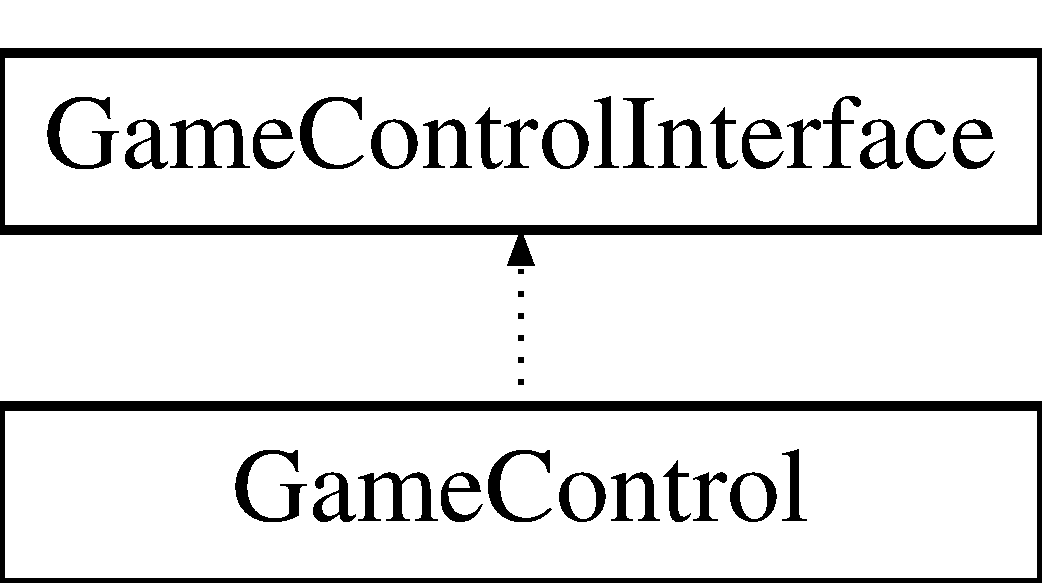
\includegraphics[height=2.000000cm]{class_game_control_interface}
\end{center}
\end{figure}
\subsection*{Public Member Functions}
\begin{DoxyCompactItemize}
\item 
virtual char {\bfseries read\+Key} ()=0\hypertarget{class_game_control_interface_ad4e7d9fbda85ecac54f7dae9f8b71a1d}{}\label{class_game_control_interface_ad4e7d9fbda85ecac54f7dae9f8b71a1d}

\item 
virtual void {\bfseries update\+Screen} ()=0\hypertarget{class_game_control_interface_a8ed7d203ab84871801b51b27da6c0459}{}\label{class_game_control_interface_a8ed7d203ab84871801b51b27da6c0459}

\item 
virtual void {\bfseries set\+Command} (C\+O\+M\+M\+A\+ND)=0\hypertarget{class_game_control_interface_a721c209eee504ff9002ac9cfefc89083}{}\label{class_game_control_interface_a721c209eee504ff9002ac9cfefc89083}

\item 
virtual C\+O\+M\+M\+A\+ND {\bfseries read\+Command} ()=0\hypertarget{class_game_control_interface_a80524b79b9791b7fa77a157b18606c61}{}\label{class_game_control_interface_a80524b79b9791b7fa77a157b18606c61}

\item 
virtual void {\bfseries send\+Command} (C\+O\+M\+M\+A\+ND)=0\hypertarget{class_game_control_interface_a700e8cfa7c588470a6be1e5870af3da7}{}\label{class_game_control_interface_a700e8cfa7c588470a6be1e5870af3da7}

\item 
virtual void {\bfseries command\+Received} ()=0\hypertarget{class_game_control_interface_aeb025f479c075181075279d34176a2cf}{}\label{class_game_control_interface_aeb025f479c075181075279d34176a2cf}

\end{DoxyCompactItemize}


The documentation for this class was generated from the following file\+:\begin{DoxyCompactItemize}
\item 
Game\+Control\+Interface.\+hpp\end{DoxyCompactItemize}

\hypertarget{class_game_data}{}\section{Game\+Data Class Reference}
\label{class_game_data}\index{Game\+Data@{Game\+Data}}
\subsection*{Public Member Functions}
\begin{DoxyCompactItemize}
\item 
int \hyperlink{class_game_data_a6266b99e1f60313355edc62ebc90b1b2}{get\+Data} (int data\+To\+Get)
\begin{DoxyCompactList}\small\item\em Get Data. \end{DoxyCompactList}\item 
void \hyperlink{class_game_data_a3e36817b28b4ef7f48c8c4a5c5d6d3b4}{set\+Data} (int data\+To\+Set, int data)
\begin{DoxyCompactList}\small\item\em Set Data. \end{DoxyCompactList}\item 
void \hyperlink{class_game_data_a16b5607cbc3200e8bad2f1495a7a9acd}{update\+Score} (int lost\+Points)
\begin{DoxyCompactList}\small\item\em Update Score. \end{DoxyCompactList}\item 
void \hyperlink{class_game_data_a05ec828c88b522f9037b3929a4d0ecd7}{update\+Time} ()
\begin{DoxyCompactList}\small\item\em Update Time. \end{DoxyCompactList}\end{DoxyCompactItemize}


\subsection{Member Function Documentation}
\index{Game\+Data@{Game\+Data}!get\+Data@{get\+Data}}
\index{get\+Data@{get\+Data}!Game\+Data@{Game\+Data}}
\subsubsection[{\texorpdfstring{get\+Data(int data\+To\+Get)}{getData(int dataToGet)}}]{\setlength{\rightskip}{0pt plus 5cm}int Game\+Data\+::get\+Data (
\begin{DoxyParamCaption}
\item[{int}]{data\+To\+Get}
\end{DoxyParamCaption}
)}\hypertarget{class_game_data_a6266b99e1f60313355edc62ebc90b1b2}{}\label{class_game_data_a6266b99e1f60313355edc62ebc90b1b2}


Get Data. 

get\+Data can be utilised to get the data specified with the integer that is given. 0 stands for\+: player\+ID 1 stands for\+: weapon 2 stands for\+: score 3 stands for\+: game\+Time \index{Game\+Data@{Game\+Data}!set\+Data@{set\+Data}}
\index{set\+Data@{set\+Data}!Game\+Data@{Game\+Data}}
\subsubsection[{\texorpdfstring{set\+Data(int data\+To\+Set, int data)}{setData(int dataToSet, int data)}}]{\setlength{\rightskip}{0pt plus 5cm}void Game\+Data\+::set\+Data (
\begin{DoxyParamCaption}
\item[{int}]{data\+To\+Set, }
\item[{int}]{data}
\end{DoxyParamCaption}
)}\hypertarget{class_game_data_a3e36817b28b4ef7f48c8c4a5c5d6d3b4}{}\label{class_game_data_a3e36817b28b4ef7f48c8c4a5c5d6d3b4}


Set Data. 

Uses the same integer values as get\+Data but can only access the player\+ID, weapon and game\+Time and sets the data accordingly. \index{Game\+Data@{Game\+Data}!update\+Score@{update\+Score}}
\index{update\+Score@{update\+Score}!Game\+Data@{Game\+Data}}
\subsubsection[{\texorpdfstring{update\+Score(int lost\+Points)}{updateScore(int lostPoints)}}]{\setlength{\rightskip}{0pt plus 5cm}void Game\+Data\+::update\+Score (
\begin{DoxyParamCaption}
\item[{int}]{lost\+Points}
\end{DoxyParamCaption}
)}\hypertarget{class_game_data_a16b5607cbc3200e8bad2f1495a7a9acd}{}\label{class_game_data_a16b5607cbc3200e8bad2f1495a7a9acd}


Update Score. 

When the score needs to be changed it can be done using this function. It will substract the amount of lost\+Points of the total value of score \index{Game\+Data@{Game\+Data}!update\+Time@{update\+Time}}
\index{update\+Time@{update\+Time}!Game\+Data@{Game\+Data}}
\subsubsection[{\texorpdfstring{update\+Time()}{updateTime()}}]{\setlength{\rightskip}{0pt plus 5cm}void Game\+Data\+::update\+Time (
\begin{DoxyParamCaption}
{}
\end{DoxyParamCaption}
)}\hypertarget{class_game_data_a05ec828c88b522f9037b3929a4d0ecd7}{}\label{class_game_data_a05ec828c88b522f9037b3929a4d0ecd7}


Update Time. 

This function gets called when there needs to be a update of the game\+Time, this will occur every second. 

The documentation for this class was generated from the following files\+:\begin{DoxyCompactItemize}
\item 
Game\+Data.\+hpp\item 
Game\+Data.\+cpp\end{DoxyCompactItemize}

\hypertarget{class_game_state_interface}{}\section{Game\+State\+Interface Class Reference}
\label{class_game_state_interface}\index{Game\+State\+Interface@{Game\+State\+Interface}}
Inheritance diagram for Game\+State\+Interface\+:\begin{figure}[H]
\begin{center}
\leavevmode
\includegraphics[height=2.000000cm]{class_game_state_interface}
\end{center}
\end{figure}
\subsection*{Public Member Functions}
\begin{DoxyCompactItemize}
\item 
virtual void {\bfseries command\+Ready\+To\+Send} (\hyperlink{class_game_control_interface}{Game\+Control\+Interface} $\ast$game\+Control)=0\hypertarget{class_game_state_interface_a6fc898f57eb2a8abb221c37fb865655e}{}\label{class_game_state_interface_a6fc898f57eb2a8abb221c37fb865655e}

\item 
virtual void {\bfseries key\+Pressed} (\hyperlink{class_game_control_interface}{Game\+Control\+Interface} $\ast$game\+Control)=0\hypertarget{class_game_state_interface_aa78a52cdc1671836db67eb403fd8de5b}{}\label{class_game_state_interface_aa78a52cdc1671836db67eb403fd8de5b}

\item 
virtual void {\bfseries data\+Changed} (\hyperlink{class_game_control_interface}{Game\+Control\+Interface} $\ast$game\+Control)=0\hypertarget{class_game_state_interface_a1c392f30c3b984180ab45f8ae5ecea80}{}\label{class_game_state_interface_a1c392f30c3b984180ab45f8ae5ecea80}

\end{DoxyCompactItemize}


The documentation for this class was generated from the following file\+:\begin{DoxyCompactItemize}
\item 
Game\+State\+Interface.\+hpp\end{DoxyCompactItemize}

\hypertarget{class_game_time_control}{}\section{Game\+Time\+Control Class Reference}
\label{class_game_time_control}\index{Game\+Time\+Control@{Game\+Time\+Control}}
Inheritance diagram for Game\+Time\+Control\+:\begin{figure}[H]
\begin{center}
\leavevmode
\includegraphics[height=2.000000cm]{class_game_time_control}
\end{center}
\end{figure}
\subsection*{Public Member Functions}
\begin{DoxyCompactItemize}
\item 
{\bfseries Game\+Time\+Control} (\hyperlink{class_game_data}{Game\+Data} \&data, \hyperlink{class_game_control}{Game\+Control} \&game\+Control)\hypertarget{class_game_time_control_a138b91b4f0c8eb315bf453c17abce316}{}\label{class_game_time_control_a138b91b4f0c8eb315bf453c17abce316}

\end{DoxyCompactItemize}


The documentation for this class was generated from the following files\+:\begin{DoxyCompactItemize}
\item 
Game\+Time\+Control.\+hpp\item 
Game\+Time\+Control.\+cpp\end{DoxyCompactItemize}

\hypertarget{class_initialize_game_state}{}\section{Initialize\+Game\+State Class Reference}
\label{class_initialize_game_state}\index{Initialize\+Game\+State@{Initialize\+Game\+State}}


The documentation for this class was generated from the following files\+:\begin{DoxyCompactItemize}
\item 
Initialize\+Game\+State.\+hpp\item 
Initialize\+Game\+State.\+cpp\end{DoxyCompactItemize}

\hypertarget{class_i_r_led}{}\section{I\+R\+Led Class Reference}
\label{class_i_r_led}\index{I\+R\+Led@{I\+R\+Led}}
\subsection*{Public Member Functions}
\begin{DoxyCompactItemize}
\item 
{\bfseries I\+R\+Led} (target\+::d2\+\_\+36k\+Hz \&diode)\hypertarget{class_i_r_led_a02838f19956f2ef4a3fb2754a2913b80}{}\label{class_i_r_led_a02838f19956f2ef4a3fb2754a2913b80}

\item 
void {\bfseries on} ()\hypertarget{class_i_r_led_ad84cfe4ff053471f6caafd720cb8a1e9}{}\label{class_i_r_led_ad84cfe4ff053471f6caafd720cb8a1e9}

\item 
void {\bfseries off} ()\hypertarget{class_i_r_led_a5780650c08a186a6b970f56d1ac78775}{}\label{class_i_r_led_a5780650c08a186a6b970f56d1ac78775}

\end{DoxyCompactItemize}


The documentation for this class was generated from the following files\+:\begin{DoxyCompactItemize}
\item 
I\+R\+Led.\+hpp\item 
I\+R\+Led.\+cpp\end{DoxyCompactItemize}

\hypertarget{class_i_r_led_controller}{}\section{I\+R\+Led\+Controller Class Reference}
\label{class_i_r_led_controller}\index{I\+R\+Led\+Controller@{I\+R\+Led\+Controller}}
Inheritance diagram for I\+R\+Led\+Controller\+:\begin{figure}[H]
\begin{center}
\leavevmode
\includegraphics[height=2.000000cm]{class_i_r_led_controller}
\end{center}
\end{figure}
\subsection*{Public Member Functions}
\begin{DoxyCompactItemize}
\item 
{\bfseries I\+R\+Led\+Controller} (\hyperlink{class_i_r_led}{I\+R\+Led} \&led)\hypertarget{class_i_r_led_controller_a4aad853ef866b522e3cf023d4b02b4c0}{}\label{class_i_r_led_controller_a4aad853ef866b522e3cf023d4b02b4c0}

\item 
void {\bfseries write\+Command} (int command)\hypertarget{class_i_r_led_controller_a42610b44fe281432ad6ebba2fb72f823}{}\label{class_i_r_led_controller_a42610b44fe281432ad6ebba2fb72f823}

\item 
void {\bfseries send\+Command} (int command)\hypertarget{class_i_r_led_controller_adeeff253be774a6a11d567110858624e}{}\label{class_i_r_led_controller_adeeff253be774a6a11d567110858624e}

\end{DoxyCompactItemize}


The documentation for this class was generated from the following files\+:\begin{DoxyCompactItemize}
\item 
I\+R\+Led\+Controller.\+hpp\item 
I\+R\+Led\+Controller.\+cpp\end{DoxyCompactItemize}

\hypertarget{class_i_r_sensor}{}\section{I\+R\+Sensor Class Reference}
\label{class_i_r_sensor}\index{I\+R\+Sensor@{I\+R\+Sensor}}
\subsection*{Public Member Functions}
\begin{DoxyCompactItemize}
\item 
{\bfseries I\+R\+Sensor} (target\+::pin\+\_\+in \&diode)\hypertarget{class_i_r_sensor_a633ce868e9539c0c45f632009b5e785c}{}\label{class_i_r_sensor_a633ce868e9539c0c45f632009b5e785c}

\item 
bool {\bfseries get} ()\hypertarget{class_i_r_sensor_a7eaba52218dcdc0f6a9e1b37ea7518fb}{}\label{class_i_r_sensor_a7eaba52218dcdc0f6a9e1b37ea7518fb}

\end{DoxyCompactItemize}


The documentation for this class was generated from the following files\+:\begin{DoxyCompactItemize}
\item 
I\+R\+Sensor.\+hpp\item 
I\+R\+Sensor.\+cpp\end{DoxyCompactItemize}

\hypertarget{class_i_r_sensor_controller}{}\section{I\+R\+Sensor\+Controller Class Reference}
\label{class_i_r_sensor_controller}\index{I\+R\+Sensor\+Controller@{I\+R\+Sensor\+Controller}}
Inheritance diagram for I\+R\+Sensor\+Controller\+:\begin{figure}[H]
\begin{center}
\leavevmode
\includegraphics[height=2.000000cm]{class_i_r_sensor_controller}
\end{center}
\end{figure}
\subsection*{Public Member Functions}
\begin{DoxyCompactItemize}
\item 
{\bfseries I\+R\+Sensor\+Controller} (\hyperlink{class_i_r_sensor}{I\+R\+Sensor} \&sensor)\hypertarget{class_i_r_sensor_controller_ac80f10a1bae68d5f70cdd749ae4c580f}{}\label{class_i_r_sensor_controller_ac80f10a1bae68d5f70cdd749ae4c580f}

\item 
C\+O\+M\+M\+A\+ND {\bfseries get\+Signal} ()\hypertarget{class_i_r_sensor_controller_aae3687a0c30ee121d371de0ac4e6ccf0}{}\label{class_i_r_sensor_controller_aae3687a0c30ee121d371de0ac4e6ccf0}

\item 
void {\bfseries store\+Signal} ()\hypertarget{class_i_r_sensor_controller_a2b14c3a18a8a0619eae667b47f0d3556}{}\label{class_i_r_sensor_controller_a2b14c3a18a8a0619eae667b47f0d3556}

\end{DoxyCompactItemize}


The documentation for this class was generated from the following files\+:\begin{DoxyCompactItemize}
\item 
I\+R\+Sensor\+Controller.\+hpp\item 
I\+R\+Sensor\+Controller.\+cpp\end{DoxyCompactItemize}

\hypertarget{class_keypad_control}{}\section{Keypad\+Control Class Reference}
\label{class_keypad_control}\index{Keypad\+Control@{Keypad\+Control}}
Inheritance diagram for Keypad\+Control\+:\begin{figure}[H]
\begin{center}
\leavevmode
\includegraphics[height=2.000000cm]{class_keypad_control}
\end{center}
\end{figure}
\subsection*{Public Member Functions}
\begin{DoxyCompactItemize}
\item 
{\bfseries Keypad\+Control} (hwlib\+::keypad$<$ 16 $>$ \&keypad, \hyperlink{class_game_control}{Game\+Control} \&game\+Control)\hypertarget{class_keypad_control_ab6a306abe67081b5cbd1973dd7db5ff5}{}\label{class_keypad_control_ab6a306abe67081b5cbd1973dd7db5ff5}

\end{DoxyCompactItemize}


The documentation for this class was generated from the following files\+:\begin{DoxyCompactItemize}
\item 
Keypad\+Control.\+hpp\item 
Keypad\+Control.\+cpp\end{DoxyCompactItemize}

\input{structldiv__t}
\hypertarget{structlldiv__t}{}\section{lldiv\+\_\+t Struct Reference}
\label{structlldiv__t}\index{lldiv\+\_\+t@{lldiv\+\_\+t}}
\subsection*{Public Attributes}
\begin{DoxyCompactItemize}
\item 
long long int {\bfseries quot}\hypertarget{structlldiv__t_aa2c189bf2a4ebe0f680463e4ce32b72f}{}\label{structlldiv__t_aa2c189bf2a4ebe0f680463e4ce32b72f}

\item 
long long int {\bfseries rem}\hypertarget{structlldiv__t_adc99c61028a27673c373ab2815f90a79}{}\label{structlldiv__t_adc99c61028a27673c373ab2815f90a79}

\end{DoxyCompactItemize}


The documentation for this struct was generated from the following file\+:\begin{DoxyCompactItemize}
\item 
bmptk\+\_\+fixed\+\_\+size\+\_\+stack.\+c\end{DoxyCompactItemize}

\hypertarget{structmax__align__t}{}\section{max\+\_\+align\+\_\+t Struct Reference}
\label{structmax__align__t}\index{max\+\_\+align\+\_\+t@{max\+\_\+align\+\_\+t}}
\subsection*{Public Member Functions}
\begin{DoxyCompactItemize}
\item 
long long \+\_\+\+\_\+max\+\_\+align\+\_\+ll {\bfseries \+\_\+\+\_\+attribute\+\_\+\+\_\+} ((\+\_\+\+\_\+aligned\+\_\+\+\_\+(\+\_\+\+\_\+alignof\+\_\+\+\_\+(long long))))\hypertarget{structmax__align__t_a9c2a8a1e8efae947243c5e8efd95123e}{}\label{structmax__align__t_a9c2a8a1e8efae947243c5e8efd95123e}

\item 
long double \+\_\+\+\_\+max\+\_\+align\+\_\+ld {\bfseries \+\_\+\+\_\+attribute\+\_\+\+\_\+} ((\+\_\+\+\_\+aligned\+\_\+\+\_\+(\+\_\+\+\_\+alignof\+\_\+\+\_\+(long double))))\hypertarget{structmax__align__t_a10d1b6c9f88535237d223c3be5232720}{}\label{structmax__align__t_a10d1b6c9f88535237d223c3be5232720}

\end{DoxyCompactItemize}


The documentation for this struct was generated from the following file\+:\begin{DoxyCompactItemize}
\item 
bmptk\+\_\+fixed\+\_\+size\+\_\+stack.\+c\end{DoxyCompactItemize}

\hypertarget{class_o_l_e_d_control}{}\section{O\+L\+E\+D\+Control Class Reference}
\label{class_o_l_e_d_control}\index{O\+L\+E\+D\+Control@{O\+L\+E\+D\+Control}}
\subsection*{Public Member Functions}
\begin{DoxyCompactItemize}
\item 
\hyperlink{class_o_l_e_d_control_ae6c2a83322fc8f8836e7206fb4d2961a}{O\+L\+E\+D\+Control} (hwlib\+::glcd\+\_\+oled\+\_\+buffered \&oled, \hyperlink{class_game_data}{Game\+Data} \&data)
\begin{DoxyCompactList}\small\item\em Constructor. \end{DoxyCompactList}\item 
void \hyperlink{class_o_l_e_d_control_a2b2561d90b65d70047f6e92920218d9b}{update\+Screen} ()
\begin{DoxyCompactList}\small\item\em Data Change. \end{DoxyCompactList}\item 
void {\bfseries data\+Changed} ()\hypertarget{class_o_l_e_d_control_a5c3b1e9b3099f49881e64e1ee7962419}{}\label{class_o_l_e_d_control_a5c3b1e9b3099f49881e64e1ee7962419}

\end{DoxyCompactItemize}


\subsection{Constructor \& Destructor Documentation}
\index{O\+L\+E\+D\+Control@{O\+L\+E\+D\+Control}!O\+L\+E\+D\+Control@{O\+L\+E\+D\+Control}}
\index{O\+L\+E\+D\+Control@{O\+L\+E\+D\+Control}!O\+L\+E\+D\+Control@{O\+L\+E\+D\+Control}}
\subsubsection[{\texorpdfstring{O\+L\+E\+D\+Control(hwlib\+::glcd\+\_\+oled\+\_\+buffered \&oled, Game\+Data \&data)}{OLEDControl(hwlib::glcd_oled_buffered &oled, GameData &data)}}]{\setlength{\rightskip}{0pt plus 5cm}O\+L\+E\+D\+Control\+::\+O\+L\+E\+D\+Control (
\begin{DoxyParamCaption}
\item[{hwlib\+::glcd\+\_\+oled\+\_\+buffered \&}]{oled, }
\item[{{\bf Game\+Data} \&}]{data}
\end{DoxyParamCaption}
)}\hypertarget{class_o_l_e_d_control_ae6c2a83322fc8f8836e7206fb4d2961a}{}\label{class_o_l_e_d_control_ae6c2a83322fc8f8836e7206fb4d2961a}


Constructor. 

Constructs an O\+L\+ED Control, the first param is the oled itself and the second param is the \hyperlink{class_game_data}{Game\+Data} from who the \hyperlink{class_o_l_e_d_control}{O\+L\+E\+D\+Control} needs to get it\textquotesingle{}s information 

\subsection{Member Function Documentation}
\index{O\+L\+E\+D\+Control@{O\+L\+E\+D\+Control}!update\+Screen@{update\+Screen}}
\index{update\+Screen@{update\+Screen}!O\+L\+E\+D\+Control@{O\+L\+E\+D\+Control}}
\subsubsection[{\texorpdfstring{update\+Screen()}{updateScreen()}}]{\setlength{\rightskip}{0pt plus 5cm}void O\+L\+E\+D\+Control\+::update\+Screen (
\begin{DoxyParamCaption}
{}
\end{DoxyParamCaption}
)}\hypertarget{class_o_l_e_d_control_a2b2561d90b65d70047f6e92920218d9b}{}\label{class_o_l_e_d_control_a2b2561d90b65d70047f6e92920218d9b}


Data Change. 

Whenever there is a data change the O\+L\+ED will update it\textquotesingle{}s data and display it on screen 

The documentation for this class was generated from the following files\+:\begin{DoxyCompactItemize}
\item 
O\+L\+E\+D\+Control.\+hpp\item 
O\+L\+E\+D\+Control.\+cpp\end{DoxyCompactItemize}

\hypertarget{class_receive_i_r_control}{}\section{Receive\+I\+R\+Control Class Reference}
\label{class_receive_i_r_control}\index{Receive\+I\+R\+Control@{Receive\+I\+R\+Control}}


The documentation for this class was generated from the following files\+:\begin{DoxyCompactItemize}
\item 
Receive\+I\+R\+Control.\+hpp\item 
Receive\+I\+R\+Control.\+cpp\end{DoxyCompactItemize}

\hypertarget{class_run_game_state}{}\section{Run\+Game\+State Class Reference}
\label{class_run_game_state}\index{Run\+Game\+State@{Run\+Game\+State}}


The documentation for this class was generated from the following files\+:\begin{DoxyCompactItemize}
\item 
Run\+Game.\+hpp\item 
Run\+Game.\+cpp\end{DoxyCompactItemize}

\hypertarget{class_send_i_r_control}{}\section{Send\+I\+R\+Control Class Reference}
\label{class_send_i_r_control}\index{Send\+I\+R\+Control@{Send\+I\+R\+Control}}


The documentation for this class was generated from the following files\+:\begin{DoxyCompactItemize}
\item 
Send\+I\+R\+Control.\+hpp\item 
Send\+I\+R\+Control.\+cpp\end{DoxyCompactItemize}

\hypertarget{class_setup_game}{}\section{Setup\+Game Class Reference}
\label{class_setup_game}\index{Setup\+Game@{Setup\+Game}}


The documentation for this class was generated from the following file\+:\begin{DoxyCompactItemize}
\item 
Setup\+State.\+hpp\end{DoxyCompactItemize}

\hypertarget{class_state_collection}{}\section{State\+Collection Class Reference}
\label{class_state_collection}\index{State\+Collection@{State\+Collection}}
\subsection*{Public Attributes}
\begin{DoxyCompactItemize}
\item 
\hyperlink{class_debug_state}{Debug\+State} {\bfseries dbstate}\hypertarget{class_state_collection_a906c67b622d68452ea020554dc69fe36}{}\label{class_state_collection_a906c67b622d68452ea020554dc69fe36}

\end{DoxyCompactItemize}


The documentation for this class was generated from the following file\+:\begin{DoxyCompactItemize}
\item 
State\+Collection.\+hpp\end{DoxyCompactItemize}

\hypertarget{class_transfer_game_score_state}{}\section{Transfer\+Game\+Score\+State Class Reference}
\label{class_transfer_game_score_state}\index{Transfer\+Game\+Score\+State@{Transfer\+Game\+Score\+State}}


The documentation for this class was generated from the following files\+:\begin{DoxyCompactItemize}
\item 
Transfer\+Game\+Score\+State.\+hpp\item 
Transfer\+Game\+Score\+State.\+cpp\end{DoxyCompactItemize}

\hypertarget{class_u_s_b}{}\section{U\+SB Class Reference}
\label{class_u_s_b}\index{U\+SB@{U\+SB}}


The documentation for this class was generated from the following files\+:\begin{DoxyCompactItemize}
\item 
U\+S\+B.\+hpp\item 
U\+S\+B.\+cpp\end{DoxyCompactItemize}

%--- End generated contents ---

% Index
\backmatter
\newpage
\phantomsection
\clearemptydoublepage
\addcontentsline{toc}{chapter}{Index}
\printindex

\end{document}
